\chapter{Appendix}
\vspace{12pt}
\section{Influence of $k$ on sensitivity to perturbations of $k$-NN graphs}

\begin{figure}[h]
  \centering
  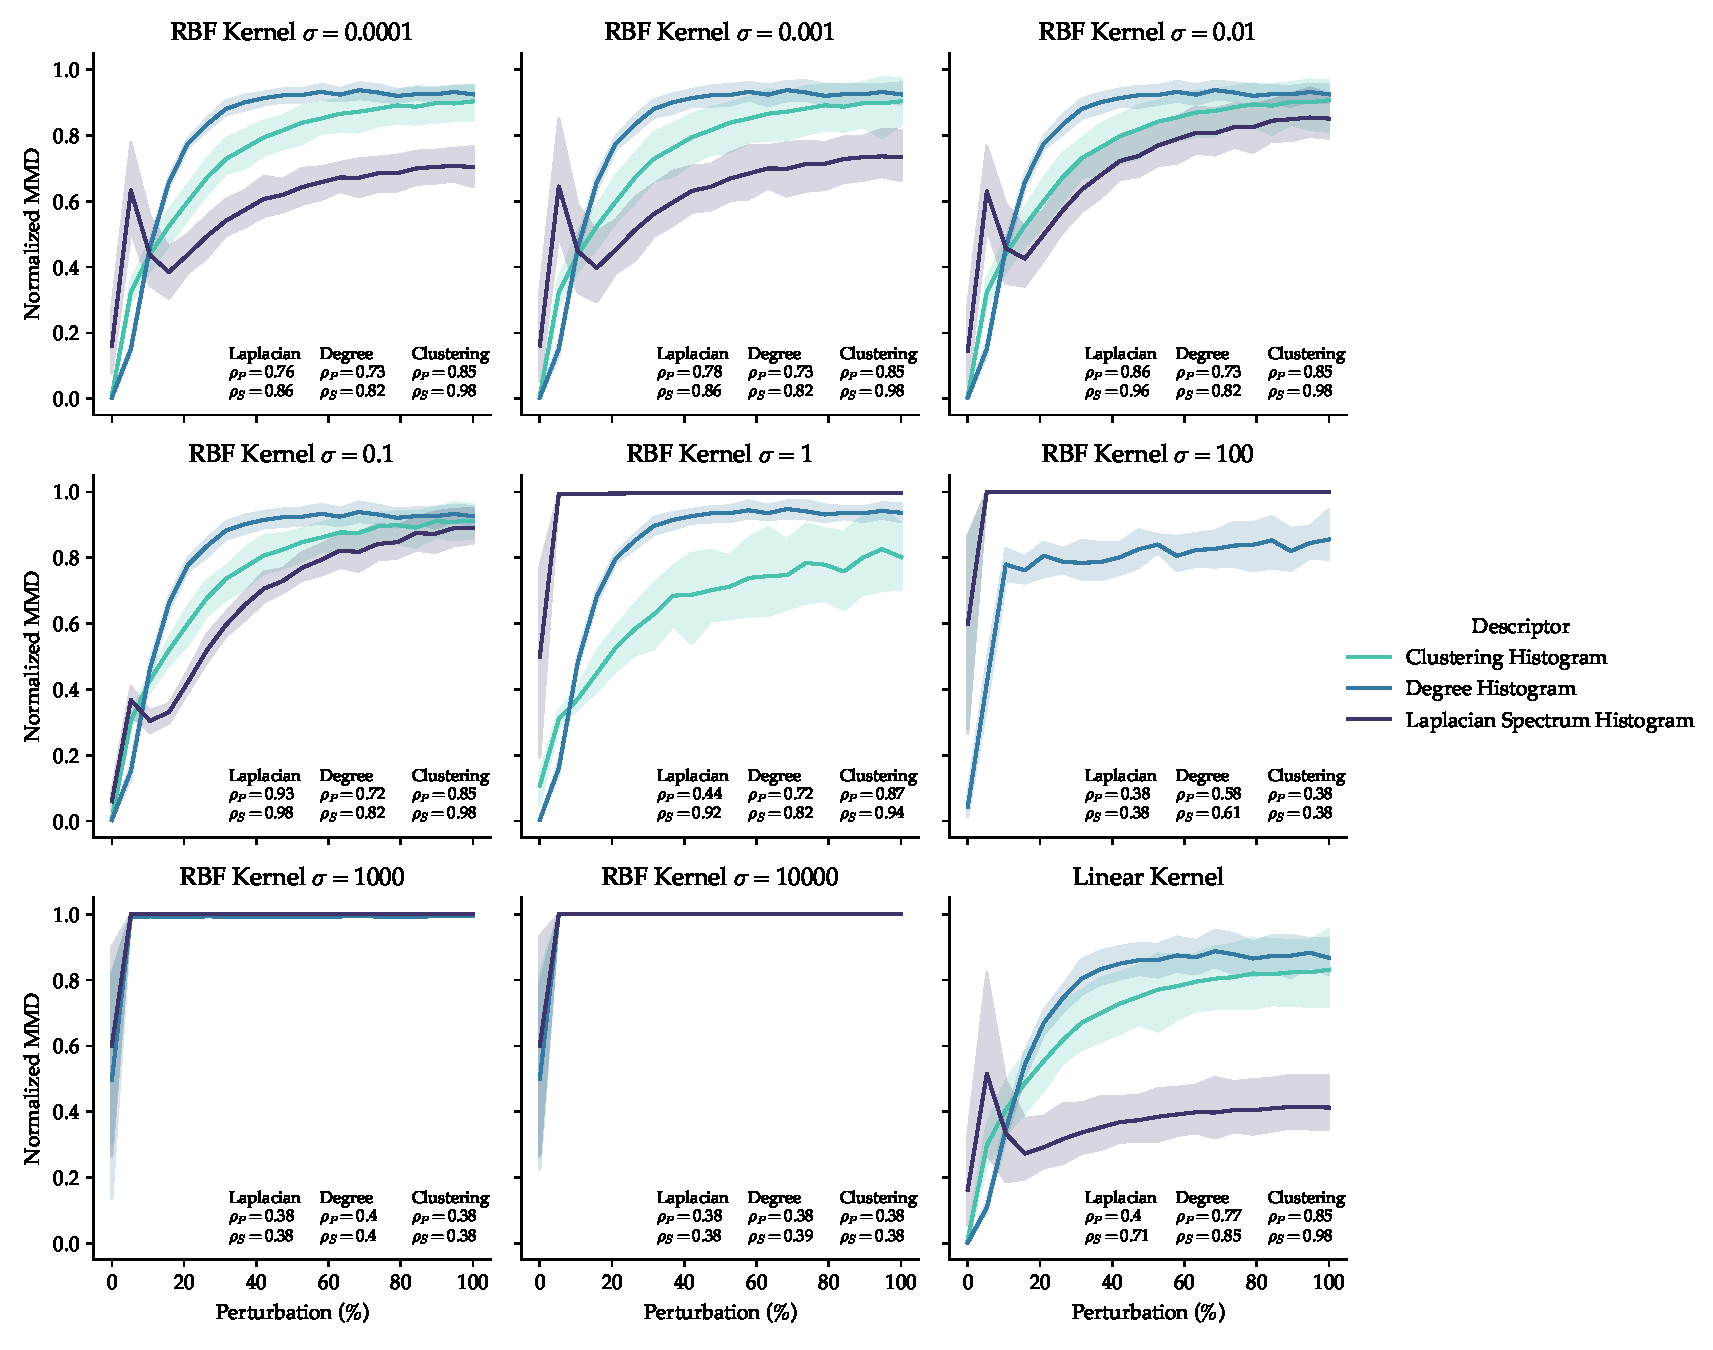
\includegraphics[width=\textwidth]{./figures/results/res_1_5.pdf}
  \caption[MMD vs. Gaussian Noise Perturbation (in \%) for various graph
descriptors of the 2-NN-graphs.]{MMD vs. Gaussian Noise Perturbation (in \%) for
various graph descriptors of the 2-NN-graphs. The kernel here is shown on top of
each subplots.}
  \label{fig:mmd_effect_kernel_knn}
\end{figure}


\section{Weisfeiler-Lehman Runtime Improvements for Sparse
  Graphs}\label{sec:sparse_wl}

In this thesis, we devised a three-pronged method to speed up the runtime of the
Weisfeiler-Lehman kernel by approximately 80\% by leveraging the sparsity of the
graphs used here. The three elements contributing to the speedup are the
following:

\begin{enumerate}
\item Our implementation parallelizes the execution of the Weisfeiler-Lehman hash
computations since each graph's hash can be computed independently prior to
computing the kernel.
\item It also parallelizes the computation of similarity of graphs in \acrshort{rkhs} by
computing batches of the inner products independently.
\item When comparing graphs, lots of CPU cycles are spent processing
positions/hashes that do not overlap between Weisfeiler-Lehman
histograms. As such, we manually loop over the overlapping keys, outperforming
NumPy dot product-based implementations on collections of sparse graphs.
\end{enumerate}

We tested, covered, and open-sourced the implementation of this novel approach
on GitHub, and is available at the following URL: \url{https://github.com/pjhartout/fastwlk}.

\section{Distance Distribution of Descriptor Functions}\label{sec:distance_dist}
To explain why certain Gaussian configurations tend to work better than others,
it is useful to compute the pairwise distance of unperturbed proteins to get an
idea of how far away in e.g. Euclidean space each embedding is from one
another. Figure \ref{fig:mean_distance_embedding} shows the pairwise Euclidean
distance distribution within an unperturbed set of proteins. We can see that
this varies quite a bit from descriptor to descriptor and that this
distribution is also affected by the parameters used to extract the graphs in
the case of graph descriptors. This probably explains why we see different
behaviors for different kernels in Figure \ref{fig:mmd_effect_kernel}.

Although we did not do so in this thesis, one could leverage this information to
set the $\sigma$ parameter for the RBF kernel by centering it around the mean,
and (logarithmically) scaling it up and down to find configurations with the
highest correlations.

\begin{figure}
  \centering
  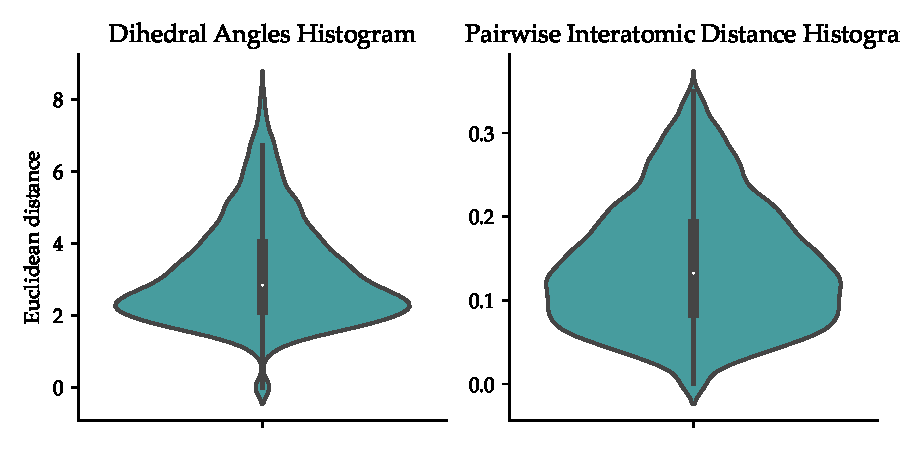
\includegraphics[width=0.6\textwidth]{./figures/results/violin_protein_descriptors.pdf}
  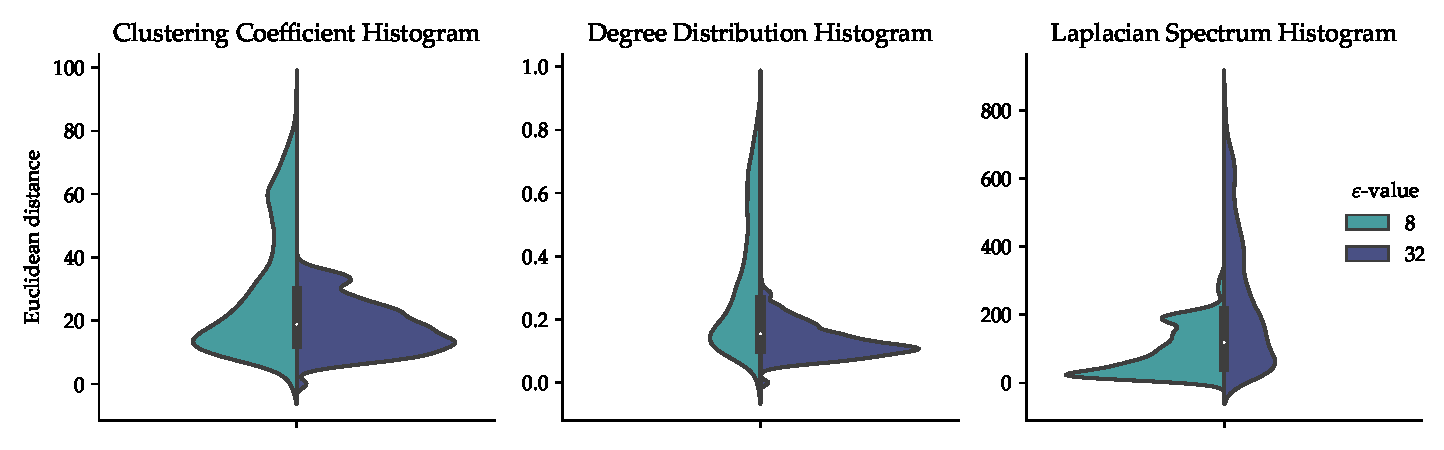
\includegraphics[width=\textwidth]{./figures/results/violin_graph_descriptors.pdf}
  \caption[Mean Euclidean distance between typical descriptor vectors used in
  this thesis]{Mean Euclidean distance between typical descriptor vectors used in
this thesis. The top row shows the mean distance between each of the protein
descriptors introduced in this thesis while the bottom row shows the distance
between each graph descriptor for two $\varepsilon$-graph extraction settings.}
  \label{fig:mean_distance_embedding}
\end{figure}

\section{MMD baselines for various configurations}\label{sec:mmd_baselines}

\acrshort{mmd} distributions between two sets of 100 unperturbed proteins with
various \acrshort{mmd} configurations are shown here. This motivates why the
practicioner should always make a positive control, as various \acrshort{mmd}
configurations can have vastly different ranges depending on the configurations.

\begin{figure}
  \centering
  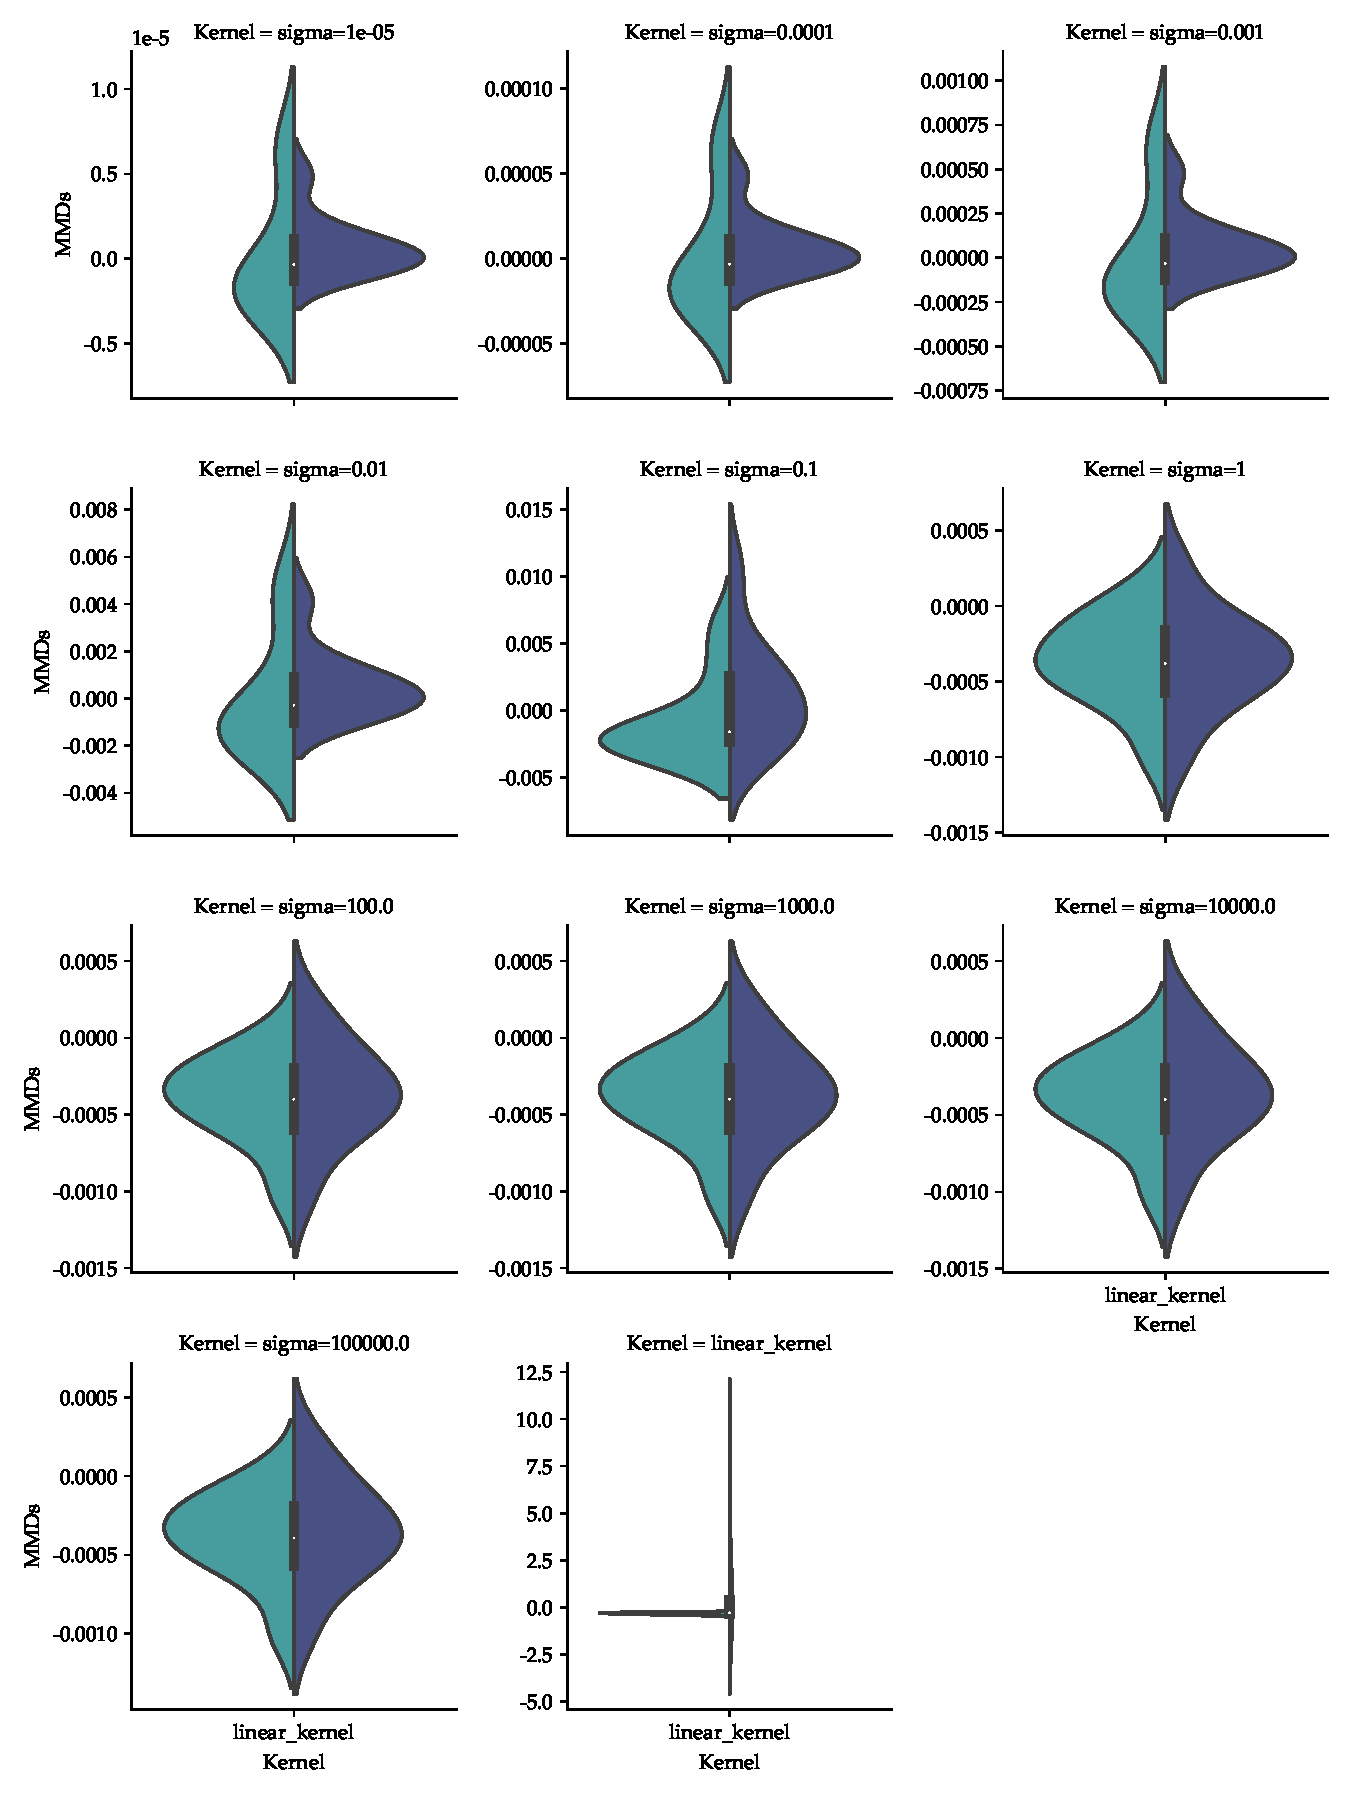
\includegraphics[width=\textwidth]{./figures/results/clustering_baselines.pdf}
  \caption[Clustering coefficient histogram \acrshort{mmd} baselines for two
different $\varepsilon$ values.]{Clustering coefficient \acrshort{mmd} baselines
for two different $\varepsilon$ values. The left side of each violin plot is
obtained with $\varepsilon=8$ and the right side with $\varepsilon=32$.
Everywhere a plot contains ``sigma'' in the title, the RBF kernel with the
indicated parameter was used.}
\end{figure}

\begin{figure}
  \centering
  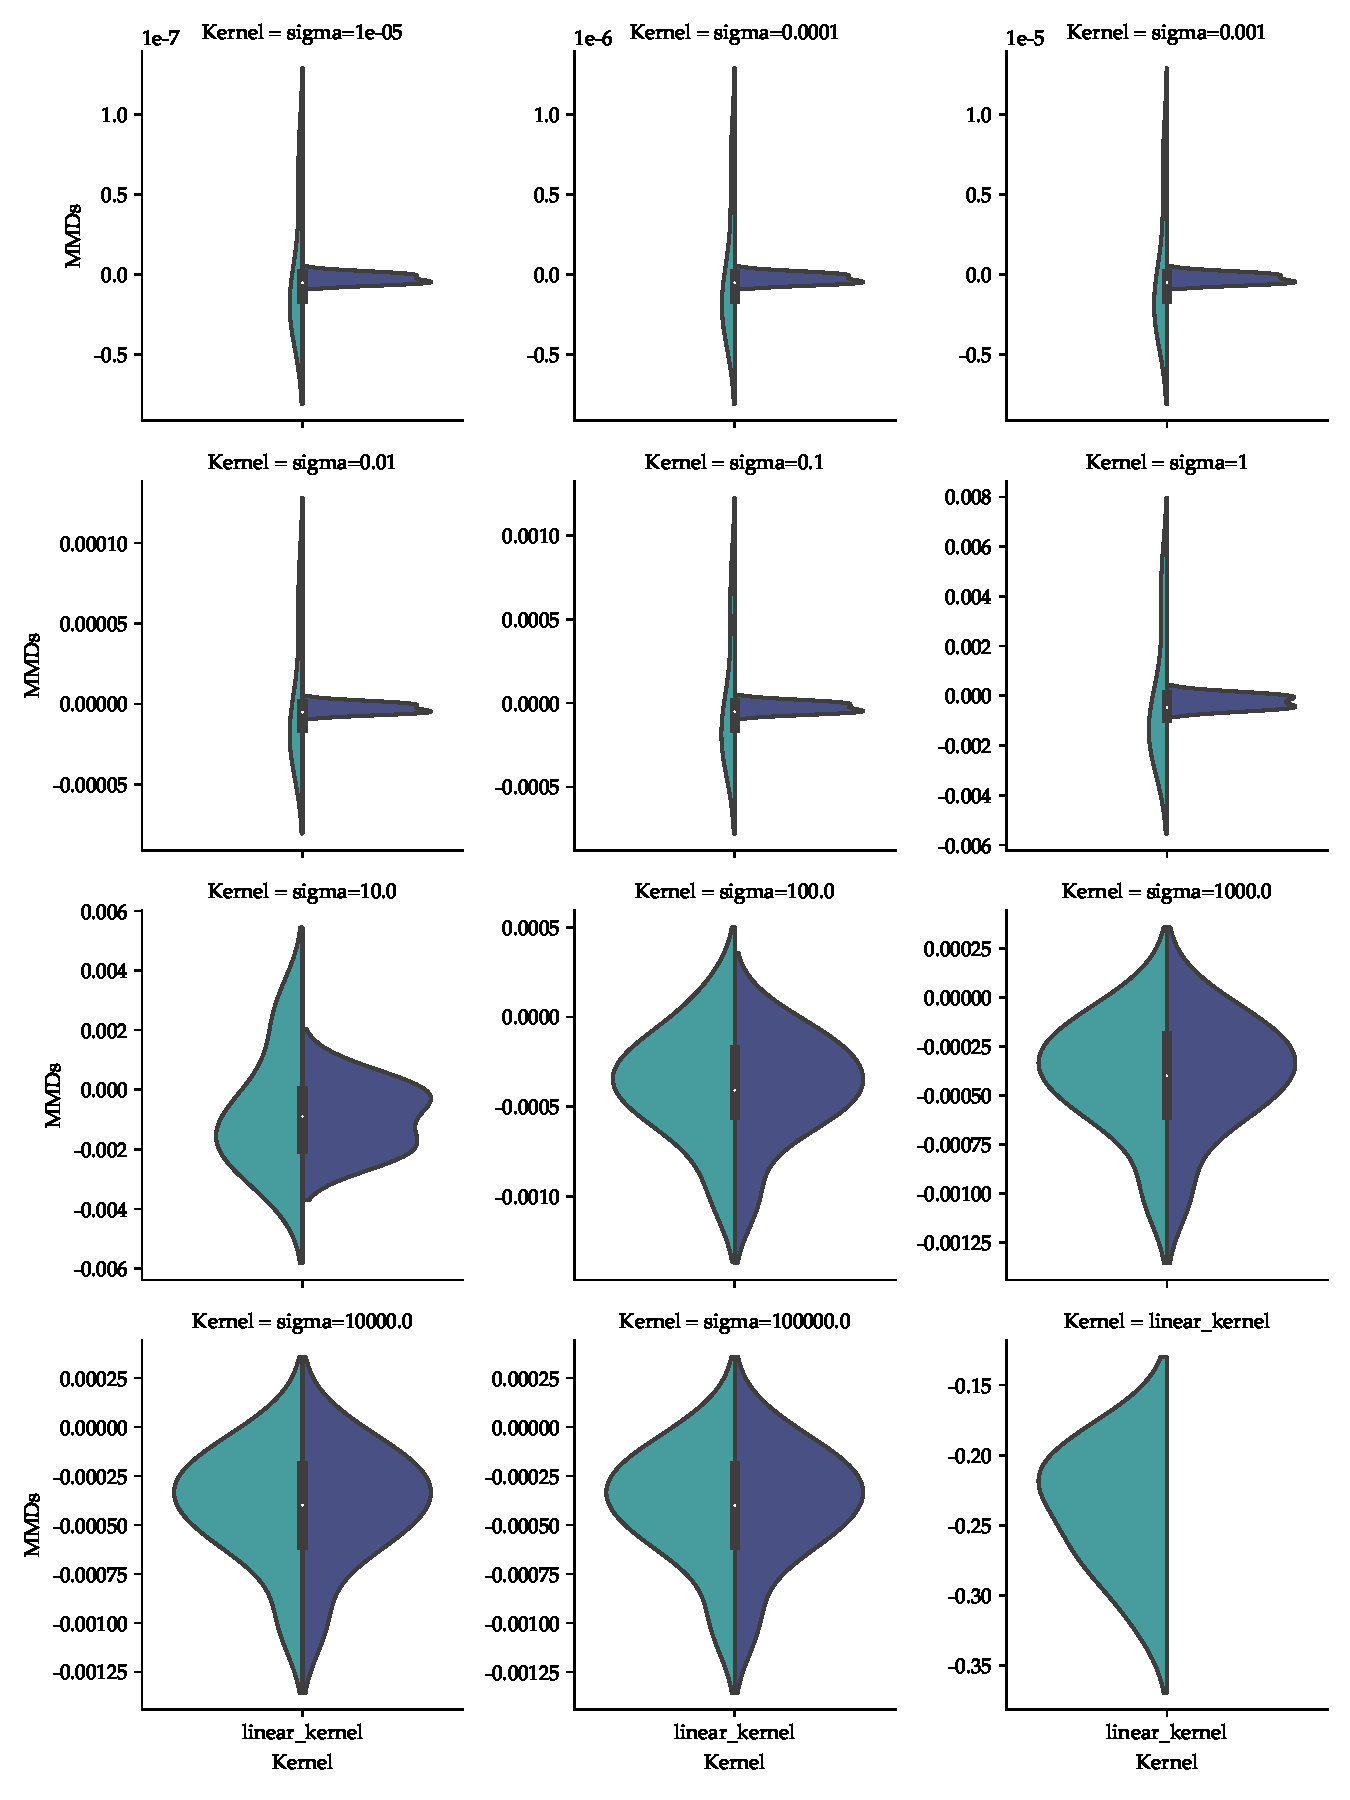
\includegraphics[width=\textwidth]{./figures/results/degree_baselines.pdf}
  \caption[Degree distribution histogram \acrshort{mmd} baselines for two
different $\varepsilon$ values.]{Degree distribution histogram \acrshort{mmd}
baselines for two different $\varepsilon$ values. The left side of each violin
plot is obtained with $\varepsilon=8$ and the right side with $\varepsilon=32$.
Everywhere a plot contains ``sigma'' in the title, the RBF kernel with the
indicated parameter was used.}
\end{figure}

\begin{figure}
  \centering
  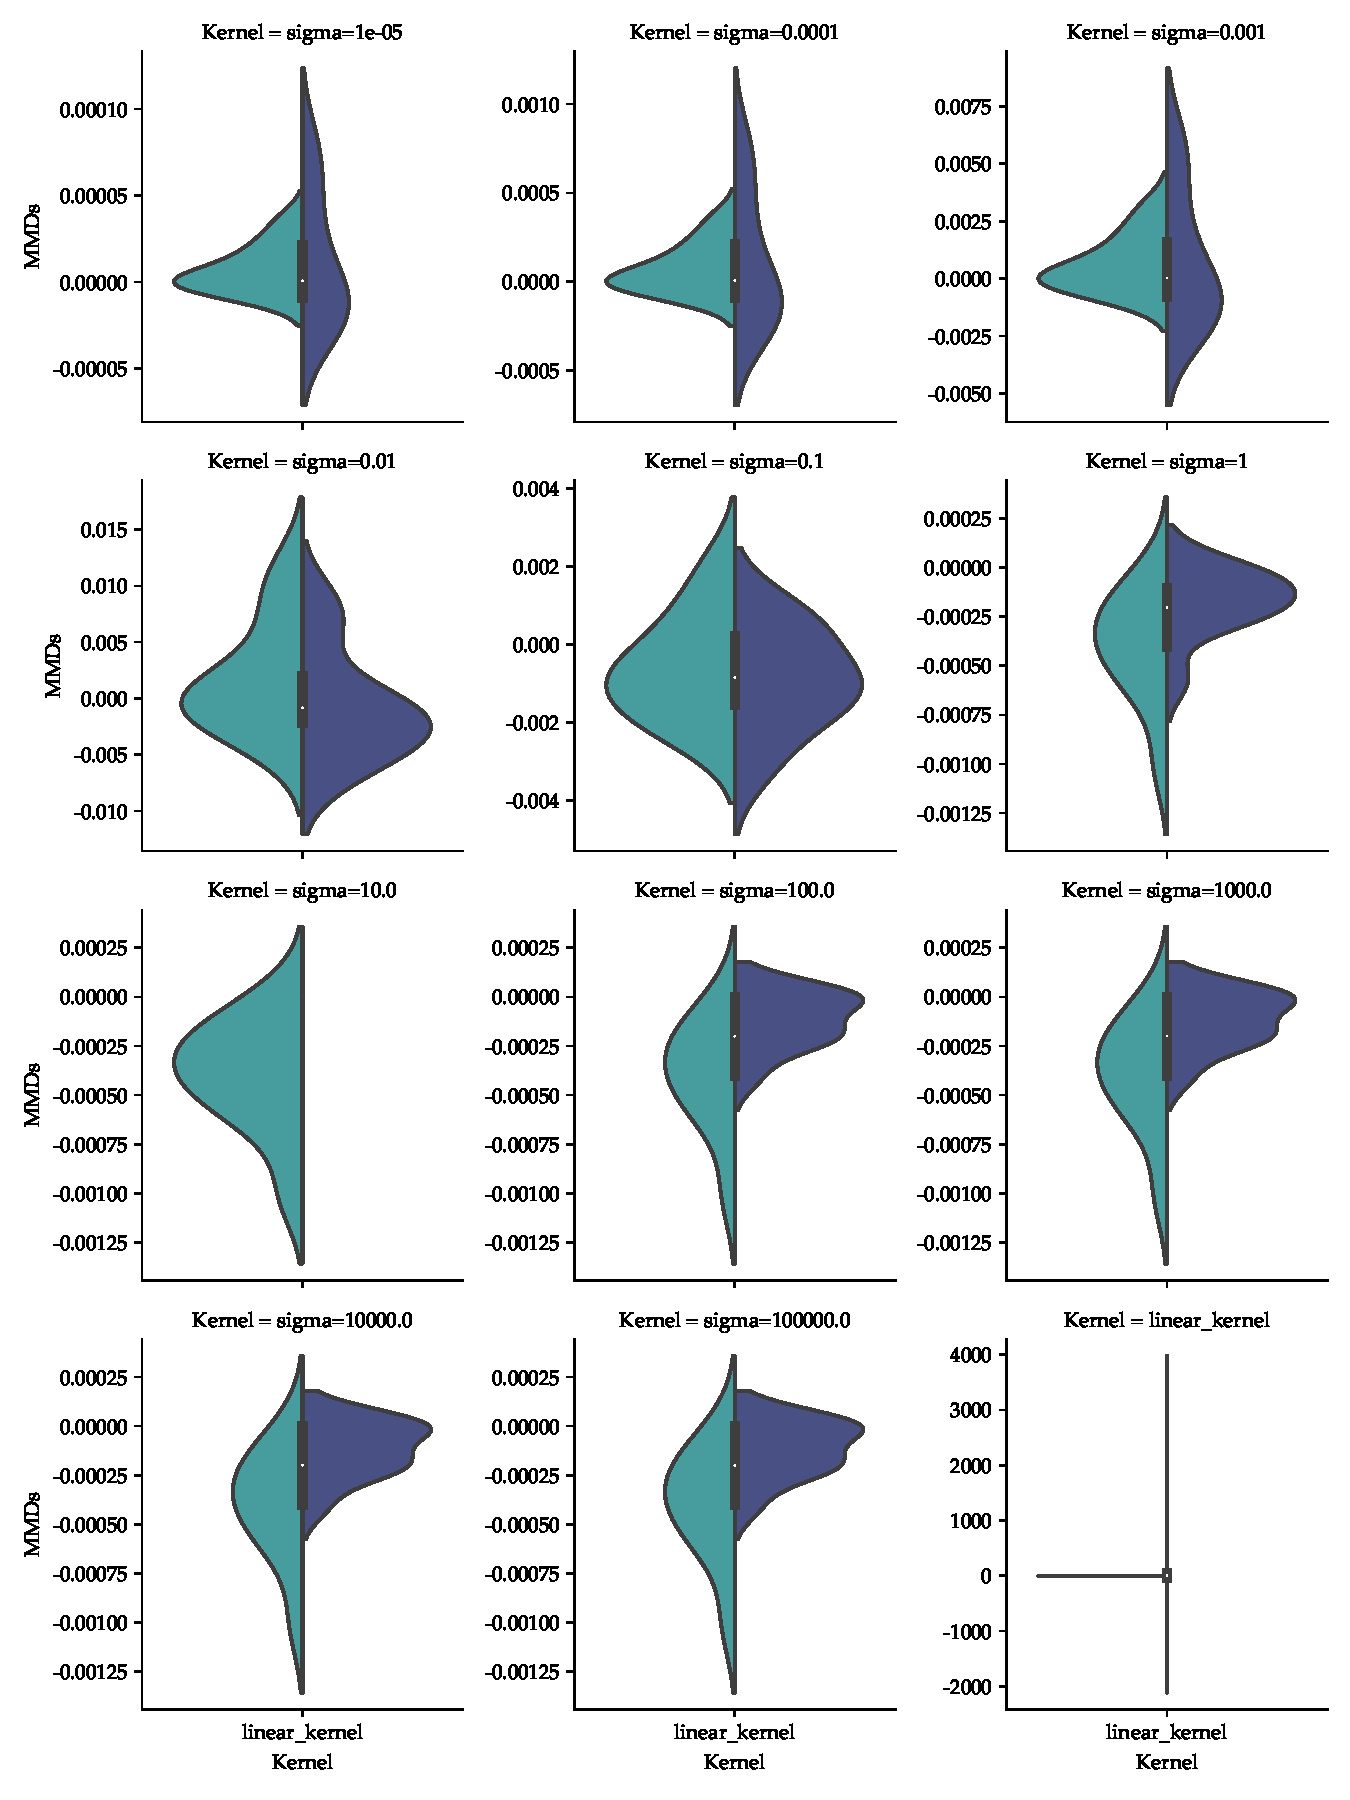
\includegraphics[width=\textwidth]{./figures/results/laplacian_spectrum_baselines.pdf}
  \caption[Laplacian spectrum histogram \acrshort{mmd} baselines for two
different $\varepsilon$ values.]{Laplacian spectrum histogram \acrshort{mmd}
baselines for two different $\varepsilon$ values. The left side of each violin
plot is obtained with $\varepsilon=8$ and the right side with
$\varepsilon=32$.Everywhere a plot contains ``sigma'' in the title, the RBF
kernel with the indicated parameter was used.}
\end{figure}

\begin{figure}
  \centering
  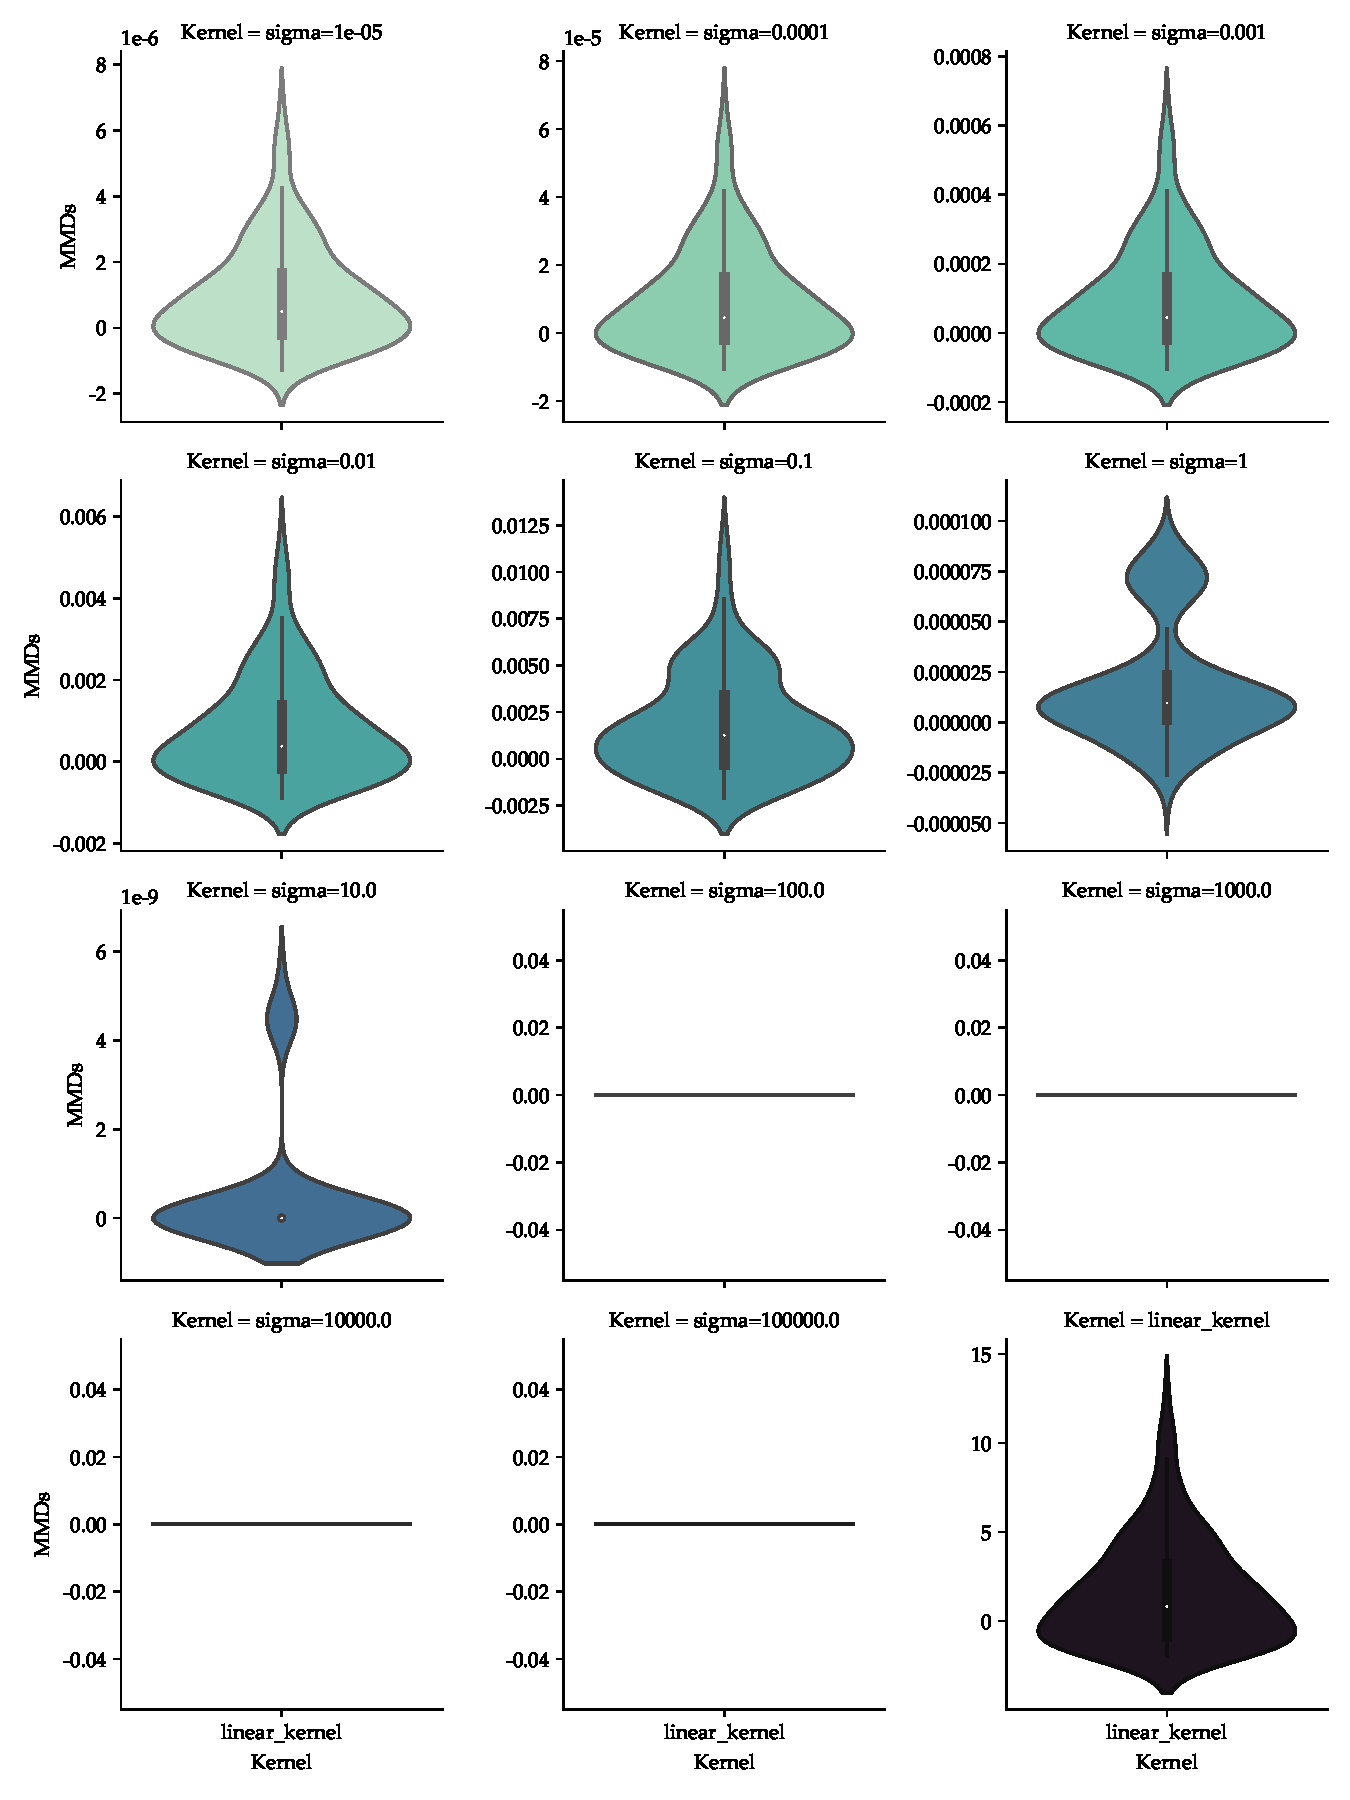
\includegraphics[width=\textwidth]{./figures/results/esm_baselines.pdf}
  \caption[\acrshort{esm}-based \acrshort{mmd} baselines for two different
$\varepsilon$ values.]{\acrshort{esm}-based \acrshort{mmd} baselines for two
different $\varepsilon$ values. The left side of each violin plot is obtained
with $\varepsilon=8$ and the right side with $\varepsilon=32$. Everywhere a plot
contains ``sigma'' in the title, the RBF kernel with the indicated parameter was
used.}
\end{figure}

\begin{figure}
  \centering
  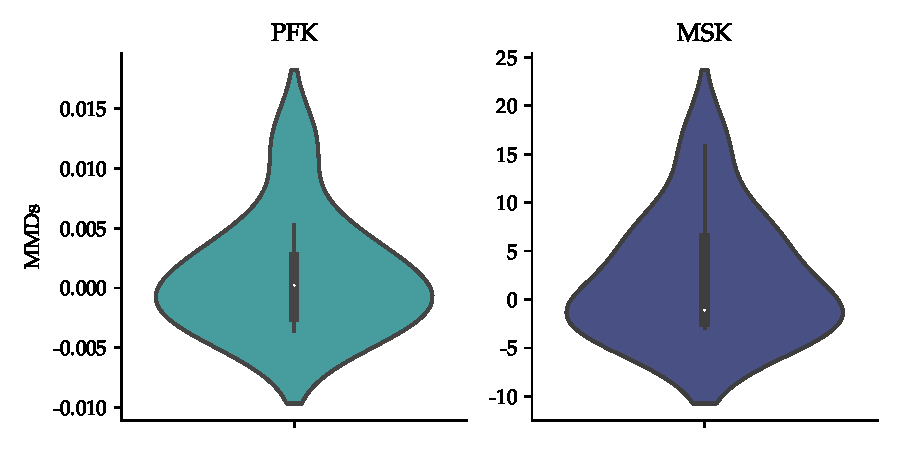
\includegraphics[width=0.6\textwidth]{./figures/results/tda_baselines.pdf}
  \caption[\acrshort{tda}-based \acrshort{mmd} baselines for two different
$\varepsilon$ values.]{\acrshort{tda}-based \acrshort{mmd} baselines for two
different $\varepsilon$ values. The left side of each violin plot is obtained
with $\varepsilon=8$ and the right side with $\varepsilon=32$. PFK: persistence
Fisher kernel. MSK: multi-scale kernel.}
\end{figure}

\begin{figure}
  \centering
  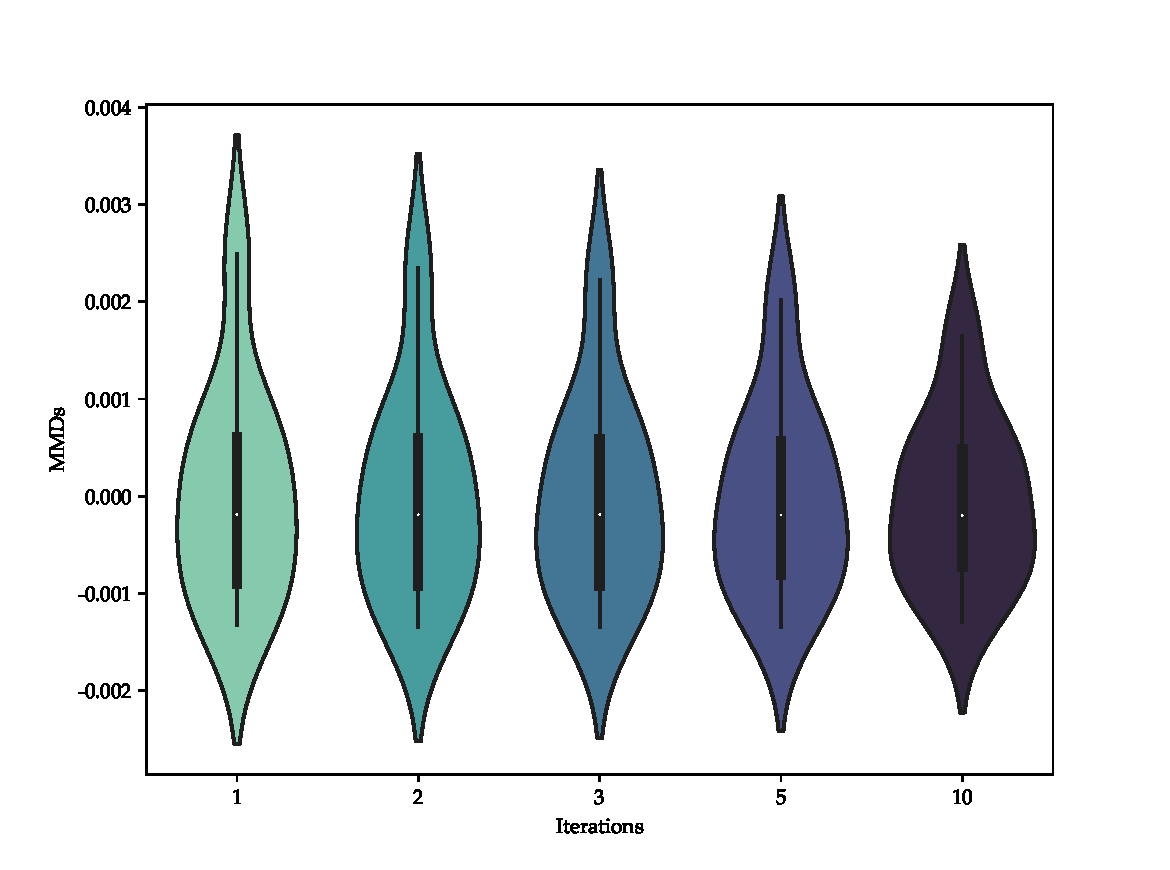
\includegraphics[width=0.75\textwidth]{./figures/results/wl_baselines.pdf}
  \caption[Weisfeiler-Lehman-based \acrshort{mmd} baselines for two different
$\varepsilon$ values.]{\acrshort{tda}-based \acrshort{mmd} baselines for two
different $\varepsilon$ values. The left side of each violin plot is obtained
with $\varepsilon=8$ and the right side with $\varepsilon=32$. PFK: persistence
Fisher kernel. MSK: multi-scale kernel. The different iterations correspond to
the different iterations of the Weisfeiler-Lehman algorithm.}
\end{figure}
